\documentclass[a4paper]{article}
\usepackage[utf8]{inputenc}
\usepackage{natbib}
\usepackage[left=2cm, right=2cm, top=2cm]{geometry}
\usepackage{graphicx}
\usepackage{multicol}
\usepackage{program}
\usepackage{indentfirst}
\usepackage{mathtools}
\usepackage{float}
\usepackage{fancyhdr}

\graphicspath{ {./images/} }

\renewcommand{\figurename}{Gambar}
\renewcommand{\refname}{REFERENSI}

\setlength{\parindent}{4em}
\setlength{\parskip}{0.5em}
\setlength{\columnsep}{1cm}

% Keywords command
\providecommand{\keywords}[1]
{
  \small	
  \textbf{\textit{Keywords ---}} #1
}

% Judul
\title{\textbf{PENGEMBANGAN \textit{FUNCTION POINT COMPLEXITY WEIGHT} DENGAN \textit{FUZZY LOGIC} METODE MAMDANI}}
\author{\textbf{Galih Dian Hutama \textsuperscript{1)} Ristu Saptono \textsuperscript{2)} Hasan Dwi Cahyono \textsuperscript{3)}}}
\date{\textsuperscript{1) 2) 3)}Informatika, FMIPA Universitas Sebelas Maret\\ Jalan Ir. Sutami 36A Kentingan, Surakarta 57126 Indonesia\\ email : \textsuperscript{1)}galihdhutama@student.uns.ac.id, \textsuperscript{2)}ristu.saptono@staff.uns.ac.id, \textsuperscript{3)}hasandc@staff.uns.ac.id}

% Header
\setlength{\headheight}{15.2pt}
\pagestyle{fancy}
\lhead{\textit{Seminar Nasional Teknologi Informasi 2015}}
\rhead{A4}

% Mulai Dokumen
\begin{document}

% Cetak Judul
\maketitle

% Bagi 2 Kolom
\begin{multicols}{2}

% Abstract
\begin{abstract}
    \textit{Measuring a software is the first step to do to build a software efficiently, effectively and give a good result. One of the part of measuring a software is by counting the software size trough Lines of Code (LOC). There are several methods for counting LOC and Function Point Analysis (FPA) is one of the method commonly used for counting LOC of a software. FPA method need to combine with another method to get a better accuracy. In this paper, fuzzy logic used to develop the weight in Function Point Complexity Table. The data is get from several applications and used as a simulation for LOC counting. LOC from FPA and fuzzy logic is being compared with real LOC of the application to get the deficit LOC. Mean Absolute Error (MAE) used as a error measuring method. The result are MAE for FPA method is 154.82 lines and MAE for FPA with fuzzy logic is 93.44 lines. This prove fuzzy logic can make LOC counting with FPA give less error which means is a better accuracy.}
\end{abstract}

% Keywords
\keywords{\textit{Lines of Code, Function Point Analisys, Fuzzy Logic.}}

% Pendahuluan
\section{PENDAHULUAN}

\par Salah satu faktor sukses dalam mengerjakan sebuah proyek, termasuk proyek perangkat lunak adalah estimasi dan perencanaan yang akan dilakukan. Proyek tidak dapat dikendalikan jika proyek tersebut tidak mempunyai estimasi dan perencanaan. Estimasi dan perencanaan dalam proyek perangkat lunak bisa diawali dengan pengukuran dari perangkat lunak yang akan dibuat atau dikembangkan. \citep{Tunali2014}

\par Ada beberapa metode dalam melakukan pengukuran perangkat lunak, salah satu yang paling banyak digunakan adalah \textit{Function Point Analysis} (FPA). FPA merupakan metode pengukuran perangkat lunak yang paling banyak digunakan di seluruh dunia. FPA pertama kali dikenalkan oleh Allan Albrecht pada tahun 1979 dan sekarang terus diperbaharui oleh \textit{International Function Point User Group} (IFPUG). Terdapat beberapa metode pengukuran perangkat lunak selain FPA, sebagai contoh : \textit{Lines of Code} (LOC) dan \textit{Wideband Delphi}. Kedua metode pengukuran perangkat lunak tersebut mempunyai beberapa issue atau permasalahan yang membuat kedua metode pengukuran perangkat lunak tersebut tidak digunakan sehingga jarang ada pengembangan yang bisa membuat kedua metode pengukuran perangkat lunak tersebut berfungsi dengan lebih baik. \par Dalam metode FPA terdapat 5 fungsi sebagai parameter pengukuran sebuah perangkat lunak, yaitu \textit{Internal Logical File} (ILF), \textit{External Interface File} (EIF), \textit{External Input} (EI), \textit{External Output} (EO), \textit{External Inquiry} (EQ). Pengukuran perangkat lunak dilakukan dengan mengambil data untuk 5 fungsi tersebut kemudian di kelompokan berdasarkan banyak Data \textit{Element Types} (DETs), \textit{File Type References} (FTRs), dan \textit{Record Element Types} (RETs) yang disebut \textit{weight} menjadi 3 kelompok, yaitu \textit{low, average,} dan \textit{high}\citep{Balaji2013}. Pengelompokan \textit{weight} tersebut sesuai dengan tabel \textit{Function Point Complexity Weight} yang dibuat oleh Allan Albrecht\citep{Xia2008}.

\par Output dari \textit{weight} yang dikelompokan berdasarkan tabel \textit{Function Point Complexity Weight} bersifat himpunan \textit{crisp} sehingga memunculkan output yang tidak sesuai antara weight yang berdekatan atau berjauhan.

\par Sebagai contoh untuk penghitungan ILF, sebuah aplikasi A memilki jumlah DET 50 dan RET 3, masuk ke kelompok \textit{average.} Aplikasi B memiliki jumlah DET 20 dan RET 3, masuk ke kelompok \textit{average.} Sedangkan aplikasi C memiliki jumlah DET 19 dan RET 3, masuk ke kelompok \textit{low.} Dengan jumlah RET yang sama untuk semua aplikasi, aplikasi A memiliki beda jumlah DET sebanyak 30 dengan aplikasi B dan kedua aplikasi tersebut masuk ke dalam kelompok yang sama, yaitu average. Sedangkan aplikasi B dan aplikasi C memiliki beda jumlah DET hanya 1 tetapi aplikasi C tidak masuk ke dalam satu kelompok dengan aplikasi B, aplikasi C masuk ke dalam kelompok \textit{low.} Ilustrasi tersebut menunjukan kelemahan himpunan \textit{crisp.} Berdasarkan pemikiran sebagai manusia, pengelompokan \textit{weight} ke dalam tabel \textit{Function Point Complexity Weight} kurang benar jika menggunakan himpunan \textit{crisp} atau nilai tunggal.

\par Dalam penelitian ini, \textit{fuzzy logic} digunakan untuk memperbaharui nilai \textit{weight} pada tabel \textit{Function Point Complexity Weight. Fuzzy logic} menghasilkan output berupa himpunan \textit{fuzzy.} Pemikiran manusia bersifat \textit{fuzzy} atau samar, begitu juga dengan kejadian real di dunia. \textit{Fuzzy logic} adalah logika yang menyatakan perkiraan bukan kepastian, yang dimana mirip dengan pemikiran manusia dan kejadian real di dunia. Oleh karena itu \textit{fuzzy logic} tidak sama seperti dengan logika pada umumnya\citep{Elamvazuthi2009}. Dengan \textit{fuzzy logic} memungkinkan adanya toleransi dalam pengelompokan nilai \textit{weight} agar memunculkan output yang lebih rasional. Sehingga \textit{output} yang didapat menjadikan pengukuran perangkat lunak lebih akurat.

\par Metode yang digunakan dalam \textit{fuzzy logic} di penelitian ini adalah metode Mamdani. Metode Mamdani telah diterima secara luas untuk digunakan para ahli dalam bidang \textit{soft computing.} Metode Mamdani bekerja lebih intuitif dan mempunyai tingkat toleransi keputusan berdasarkan pola pikir manusia yang tinggi\citep{Kaur2012}. Output dalam proses \textit{defuzifikasi} metode Mamdani berupa nilai ganda atau \textit{range} sehingga memungkinkan metode Mamdani untuk menghasilkan output yang mempunyai toleransi tinggi karena mempertimbangkan nilai-nilai didekatnya. Penerapan \textit{fuzzy logic} metode Mamdani dalam proses mendapatkan nilai weight pada tabel \textit{Function Point Complexity Weight} membuat nilai \textit{weight} yang didapat lebih akurat dan lebih sesuai.

\par Setelah mendapatkan nilai \textit{Function Point} (FP) dari sebuah perangkat lunak, maka dapat diukur \textit{size} dari perangkat lunak tersebut dengan menghitung \textit{Lines of Code} (LOC). Oleh karena itu, pengerjaan proyek perangkat lunak akan berjalan lebih efektif dan efisien dari estimasi yang didapat menggunakan FPA dengan memperbaharui \textit{weight} pada tabel \textit{Function Point Complexity Weight} menggunakan \textit{fuzzy logic} metode Mamdani.

% Dasar Teori
\section{DASAR TEORI}

\subsection{\textit{Software Size Estimation}}

\par \textit{Software Size Estimation} merupakan pembelajaran untuk memperkirakan ukuran suatu perangkat lunak yang akan dikembangkan atau dibuat. Pengukuran perangkat lunak penting agar dalam pengerjaan perangkat lunak tidak membuang percuma resource yang ada dan menggunakannya semaksimal mungkin untuk mendapatkan proses pengerjaan yang efektif dan efisien. Ada beberapa metode dalam mengukur perangkat lunak, diantaranya :

\begin{itemize}
  \item \textit{Lines of Code} (LOC)
  \item \textit{The Blitz}
  \item \textit{Wideband Delphi}
  \item \textit{Function Points}
  \item \textit{Feature Points}
  \item \textit{Object Points}
  \item \textit{Number of Boxes on a Data Flow Diagram}
  \item \textit{Number of Classes in a Design Diagram}
\end{itemize}

\par Meskipun ada banyak metode pengukuran perangkat lunak tetapi sulit untuk mendapatkan tingkat akurasi sebesar 100 persen untuk setiap metode. Diperlukan perpaduan metode untuk mendapatkan tingkat akurasi pengukuran perangkat lunak yang besar.

\subsection{\textit{Function Point Analysis}}

\par \textit{Function Point Analysis} (FPA) merupakan metode untuk mengukur pengembangan atau pembuatan perangkat lunak berdasarkan jumlah fungsionalitas dan komplesitas dari pandangan user. FPA diperkenalkan pada tahun 1986 oleh \textit{International Function Point User Group} (IFPUG). IFPUG juga membuat \textit{Counting Practices Manual} (CPM) sebagai standar industri dalam menggunakan FPA \citep{Tunali2014}. 

\par Didalam FPA terdapat 5 fungsi pembeda yang menjadi pengitungan awal mendapatkan nilai \textit{weight.} 5 fungsi tersebut adalah \citep{Pradani2013} :

\begin{itemize}
  \item \textit{Internal Logical Files} (ILF) merupakan data atau informasi kontrol yang perlu dipelihara melalui pengaksesan \textit{insert, update,} dan \textit{delete} di dalam sistem aplikasi.
  \item\textit{External Interface Files} (EIF) merupakan data atau informasi kontrol yang diperlukan oleh sistem aplikasi, tetapi disimpan atau diplehara diluar sistem oleh sistem lain.
  \item \textit{External Input} (EI) merupakan proses elementer yang memproses data dari luar sistem dan menyimpan hasilnya ke dalam sistem.
  \item \textit{External Output} (EO) merupakan proses elementer yang memproses data dan menyajikan informasi ke luar sistem dengan disertai proses komputasi atau kalkulasi ketika menyajikan informasi.
  \item \textit{External Inquiry} (EQ) merupakan proses elementer yang menyajikan data ke luar sistem tanpa melakukan proses pengolahan data.
\end{itemize}

\par Penghitungan nilai ILF, EIF, EI, EQ, dan EO juga dipengaruhi oleh tingkat kompleksitas komponen-komponen tersebut. Pengkategorian komponen didasarkan pada penghitungan DET, RET, dan FTR yang rinciannya sebagai berikut \citep{Pradani2013} :

\begin{itemize}
    \item \textit{Data Element Type} (DET) adalah elemen data yang dikenal oleh user dan merupakan \textit{non repeatable data field.} Contoh : Nama Pelanggan, Nomor Pelanggan, Tanggal Lahir, dan lain-lain.
    \item \textit{Record Element Type} (RET) adalah \textit{subgroup} data yang dikenal oleh user. Contoh: data pelanggan terdiri dari biodata, data finansial, dan data tanggungan keluarga, dan lain-lain.
    \item \textit{File Type Reference} (FTR) adalah ILF atau EIF yang dibaca atau diakses oleh proses elementer, yaitu EI, EQ, dan EO.
\end{itemize}

\par Dengan melakukan penghitungan ILF, EIF, EI, EQ, dan EO maka didapat nilai dari \textit{Unadjusted Function Point} (UFP). Terdapat 14 faktor yang berfungsi sebagai hasil perkalian untuk menjadikan UFP menjadi \textit{Function Point} (FP). 14 Faktor tersebut adalah \citep{Pradani2013} :

\begin{itemize}
    \item \textit{Data Communications} merupakan tingkat kebutuhan komunikasi langsung antara aplikasi dengan processor.
    \item \textit{Distributed Functions} merupakan tingkat kebutuhan transfer data antara komponen-komponen aplikasi.
    \item \textit{Performances Objectives} merupakan tingkat response time dan throughput yang perlu dipertimbangkan dalam pengembangan aplikasi.
    \item \textit{Heavily Used Configuration} merupakan tingkat kebutuhan dimana setting konfigurasi komputer berpengaruh terhadap pengembangan aplikasi.
    \item \textit{Transaction Rate} merupakan tingkat transaksi bisnis yang berpengaruh terhadap pengembangan aplikasi.
    \item \textit{On Line Data Entry} merupakan tingkat kebutuhan input data secara interaktif.
    \item \textit{End User Efficiency} merupakan tingkat kemudahan penggunaan aplikasi.
    \item \textit{On Line Update} merupakan tingkat kebutuhan ILF di update secara interaktif.
    \item \textit{Complex Processing} merupakan tingkat kesulitan logika proses yang mempengaruhi proses development.
    \item \textit{Reusability} merupakan tingkat kebutuhan aplikasi dan kode program dirancang dan dikembangkan untuk bisa digunakan pada aplikasi lain.
    \item \textit{Installation Ease} merupakan tingkat kemudahan konversi ke sistem baru yang berpengaruh pada proses development.
    \item \textit{Operational Ease} merupakan tingkat kemudahan aplikasi dalam aspek-aspek operasional, seperti startup, backup, dan proses recovery.
    \item \textit{Multiple Sites} merupakan tingkat kebutuhan aplikasi dapat dioperasionalkan pada lingkungan hardware dan software yang berbeda-beda.
    \item \textit{Facilitate Change} merupakan tingkat kemudahan aplikasi untuk modifikasi logika proses maupun struktur data.
\end{itemize}

\par Setelah didapatkan nilai FP, dapat dilakukan pengukuran pula terhadap \textit{size, effort,} dan \textit{resource} yang dibutuhkan dari perangkat lunak yang akan dikembangkan atau dibuat.

\subsection{\textit{Fuzzy Logic}}

\par \textit{Fuzzy logic} adalah peningkatan dari logika Boolean yang berhadapan dengan konsep kebenaran sebagian. Saat logika Boolean menyatakan bahwa segala hal dapat di ekspresikan dalam istilah biner (0 atau 1, hitam atau putih, ya atau tidak), \textit{fuzzy logic} menggantikan kebenaran Boolean dengan tingkat kebenanaran \citep{Naba2009}.

\par Himpunan \textit{fuzzy logic} pertamakali diperkenalkan oleh Lotfi A. Zadeh pada tahun 1965 sebagai cara matematis untuk merepresentasikan ketidakpastian linguistik. Berdasarkan konsep \textit{fuzzy logic}, faktor-faktor dan kriteria-kriteria dapat diklasifikasikan tanpa batasan yang mengikat. \textit{Fuzzy logic} sangat berguna untuk menyelesaikan banyak permasalahan dalam berbagai bidang yang biasanya memuat derajat ketidakpastian \citep{Gokmen2010}. Logika benar dan salah dari logika Boolean tidak dapat mengatasi masalah gradasi yang berada pada dunia nyata. Tidak seperti logika boolean, \textit{fuzzy logic} mempunyai nilai yang berkelanjutan. \textit{Fuzzy logic} dinyatakan dalam derajat dari suatu keanggotaan dan derajat dari kebenaran. Oleh sebab itu sesuatu dapat dikatakan sebagian benar dan sebagian salah pada waktu yang sama. 

\par \textit{Fuzzy logic} merupakan generalisasi dari logika Boolean yang hanya memiliki dua nilai keanggotaan yaitu 0 dan 1. Dalam \textit{fuzzy logic} nilai kebenaran suatu pernyataan berkisar dari sepenuhnya benar sampai dengan sepenuhnya salah \citep{Meimaharani2014}. \textit{Fuzzy logic} berhubungan dengan ketidakpastian yang telah menjadi sifat alamiah manusia. \textit{Fuzzy logic} memungkinkan nilai akhir berupa benar dan salah atau hitam dan putih, tetapi melibatkan area abu-abu.

\subsection{\textit{Fuzzy Inference System} Mamdani}

\par Metode Mamdani sering juga dikenal dengan nama Metode Max-Min. Metode ini diperkenalkan oleh Ebrahim Mamdani pada tahun 1975. Untuk mendapatkan output diperlukan 4 tahapan \citep{Hermawan2014}, yaitu:

\begin{itemize}
    \item Pembentukan Himpunan \textit{Fuzzy} (Fuzzifikasi)
\end{itemize}

\par Himpunan \textit{fuzzy} merupakan suatu pengembangan lebih lanjut tentang konsep himpunan dalam matematika. Himpunan \textit{fuzzy} adalah rentang dari nilai-nilai. Masing-masing nilai mempunyai derajat keanggotaan (\textit{membership}) antara 0 sampai dengan 1. Ungkapan logika Boolean menggambarkan nilai-nilai “benar” atau “salah”. \textit{Logika fuzzy} menggunakan ungkapan misalnya: “sangat lambat”, ”sedang”, “sangat cepat” dan lain-lain untuk mengungkapkan derajat intensitasnya.

\par Logika \textit{fuzzy} menggunakan satu set aturan untuk menggambarkan perilakunya. Aturan-aturan tersebut menggambarkan kondisi yang diharapkan dan hasil yang diinginkan dengan menggunakan fungsi IF… THEN. Suatu himpunan \textit{fuzzy} A dalam semesta pembicaraan dinyatakan dengan fungsi keanggotaan (\textit{membership function}) mu A, yang nilainya berada dalam interval [0,1]. Secara matematika hal ini dinyatakan dengan:

\begin{equation}
    \mu_{A} : \cup \rightarrow [0,1] ... (1)
\end{equation}

\par Himpunan \textit{fuzzy} A dalam semesta pembicaraan U biasa dinyatakan sebagai sekumpulan pasangan elemen u dan besarnya derajat keanggotaan (\textit{grade of membership}) elemen tersebut sebagai berikut:

\begin{equation}
    A = {(\upsilon, \mu_{A}(\upsilon))/\upsilon \in \cup}  ... (2)
\end{equation}

\par Tanda "/" digunakan untuk menghubungkan sebuah elemen dengan derajat keanggotaannya.

\begin{itemize}
    \item Komposisi Aturan
\end{itemize}

\par Tidak seperti penalaran monoton, apabila sistem terdiri dari beberapa aturan, maka inferensi diperoleh dari kumpulan dan korelasi antar aturan. Ada 3 metode yang digunakan dalam melakukan inferensi sistem \textit{fuzzy,} yaitu: \textit{max, additive} dan \textit{probabilistik} OR (probor).

\begin{itemize}
    \item Penegasan (Defuzzifikasi)
\end{itemize}

\par Input dari proses defuzzifikasi adalah suatu himpunan \textit{fuzzy} yang diperoleh dari komposisi aturan-aturan \textit{fuzzy,} sedangkan output yang dihasilkan merupakan suatu bilangan pada domain himpunan \textit{fuzzy} tersebut. Sehingga jika diberikan suatu himpunan \textit{fuzzy} dalam \textit{range} tertentu, maka dapat diambil suatu nilai \textit{crisp} tertentu sebagai output. Dalam metode Mamdani digunakan fungsi \textit{Center of Gravity} (COG) untuk pengambilan nilai \textit{crisp} tersebut. Formulasi untuk COG seperti dibawah ini:

\begin{equation}
    Z_{cog} = \frac{\int_{z}^{1}\mu_{A}(z)zdz}{\int_{z}^{1}\mu_{A}(z)dz}
\end{equation}
dimana mu A(z) adalah nilai \textit{agregat} berdasarkan \textit{rule} yang telah dibuat dari nilai input.

\subsection{\textit{Mean Absolute Error} (MAE)}

\par Metode \textit{Mean Absolute Error} (MAE) digunakan untuk menghitung \textit{error} tiap metode. Semakin kecil nilai MAE yang didapat maka semakin kecil pula \textit{error} yang dihasilkan metode tersebut. Formulasi metode MAE seperti dibawah ini:

\begin{equation}
   MAE = \frac{1}{n}\sum_{i=1}^{n} \left\lvert x_{i}-y_{i} \right\rvert
\end{equation}
dimana n adalah banyak item yang dihitung, x merupakan nilai prediksi dan y adalah nilai real.

% Metodologi Penelitian
\section{METODOLOGI PENELITIAN}

\begin{figure}[H]
    \centering
    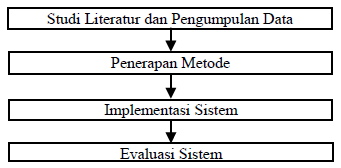
\includegraphics[width=8cm]{gambar1metodologipenelitian.png}
    \caption{Metodologi Penelitian}
    \label{gb1}
\end{figure}

\subsection{Studi Literatur dan Pengumpulan Data}

\par Studi literatur dilakukan dengan membaca sejumlah jurnal baik nasional maupun internasional. Jurnal yang dibaca adalah jurnal dengan metode yang berkaitan dengan FPA dan \textit{fuzzy logic}. Studi literatur juga bisa dilakukan dengan mempelajari modul-modul perkuliahan yang berkaitan dengan FPA dan \textit{fuzzy logic} dari berbagai Universitas. 

\par Survey dan pengumpulan data diambil dari beberapa aplikasi yang dibuat dalam Kerja Praktek Mahasiswa S1 Informatika UNS angkatan 2011 dan aplikasi yang dipakai oleh Pemerintah Kabupaten Surakarta. Dalam aplikasi tersebut diambil data berupa komponen-komponen penghitungan metode FPA sehingga dapat menentukan size dari aplikasi berdasarkan metode FPA.

\subsection{Penerapan Metode}

\par Langkah pertama melakukan perbaikan nilai \textit{weight} dengan \textit{fuzzy logic} Metode Mamdani. Nilai \textit{weight} dalam metode FPA didapat dari menghitung banyak RET/FTR dan DET yang kemudian masuk ke salah satu kelompok (\textit{low, average, high}) terlihat pada Tabel 1.

\begin{table}[H]
    \centering
    \caption{\textit{Complexity Matrix for ILF and EIF} \citep{Jones2008}}
    \bigskip
    \begin{tabular}{|c|c|c|c|}
        \hline
        \textbf{ILF/EIF} & \multicolumn{3}{|c|}{DET}\\
        \hline
        RET & 1-19 & 20-50 & 51+\\
        1 & Low & Low & Average\\
        2-5 & Low & Average & High\\
        6+ & Average & High & High\\
        \hline
    \end{tabular}
    \label{tab1}
\end{table}

\par Kemudian untuk tiap kelompok di tiap komponen memiliki nilai yang berbeda yang menjadi nilai \textit{weight} seperti terlihat pada Tabel 2.

\begin{table}[H]
    \centering
    \caption{\textit{Function Point Complexity Weight} \citep{Jones2008}}
    \bigskip
    \begin{tabular}{|c|c|c|c|}
        \hline
        \textbf{Component} & \textbf{Low} & \textbf{Average} & \textbf{High}\\
        \hline
        External Inputs & 3 & 4 & 6\\
        External Outputs & 4 & 5 & 7\\
        External Inquiris & 3 & 4 & 6\\
        Internal Logical & 7 & 10 & 15\\
        External Interface & 5 & 7 & 10\\
        \hline
    \end{tabular}
    \label{tab2}
\end{table}

\par Proses pengelompokan tersebut bersifat \textit{crisp} sehingga akan diubah dengan \textit{fuzzy logic} metode Mamdani. Pertama untuk proses fuzifikasi adalah membuat input \textit{fuzzy sets} untuk RET/FTR dan DET. Didefinisikan sebagai \textit{small, medium, large.} Didalam penelitian ini digunakan 2 model \textit{fuzzy sets.} Kemudian membuat rule untuk semua model \textit{fuzzy logic} dimana input RET/FTR dan DET dihubungkan dengan “\textit{AND}” dan menghasilkan \textit{output.} Terdapat 9 \textit{rule} seperti yang terlihat pada Tabel 3.

\begin{table}[H]
    \centering
    \caption{\textit{Fuzzy Logic Rule Set}}
    \bigskip
    \begin{tabular}{|c|c|c|c|}
        \hline
        \textbf{Rule} & \textbf{DET} & \textbf{RET/FTR} & \textbf{Output}\\
        \hline
        1 & Small & Small & Low\\
        2 & Small & Medium & Low\\
        3 & Small & Large & Average\\
        4 & Medium & Small & Low\\
        5 & Medium & Medium & Average\\
        6 & Medium & Large & High\\
        7 & Large & Small & Average\\
        8 & Large & Medium & High\\
        9 & Large & Large & High\\
        \hline
    \end{tabular}
    \label{tab3}
\end{table}

\par Kemudian proses \textit{defuzifikasi} dengan metode Mamdani menggunakan fungsi \textit{Center of Gravity} (COG). Hasil dari proses defuzifikasi tersebut merupakan nilai \textit{weight} yang baru dan digunakan untuk penghitungan metode FPA. 

\par Setelah mendapat nilai \textit{weight} yang baru dengan \textit{fuzzy logic} metode Mamdani maka dilakukan penghitungan pengukuran perangkat lunak dengan FPA. Diawali dengan mendapatkan \textit{Unadusted Function Point} (UFP) dengan cara mengalikan nilai \textit{weight} dengan jumlah fitur yang ada di setiap fungsi yang berbeda. Kemudian hasil yang didapat setiap fungsi dijumlahkan dan didapat nilai UFP.

\par Kemudian mencari nilai \textit{Total Degree of Infulence} (TDI) dengan cara menjumlahkan banyak pengaruh terhadap perangkat lunak yang diukur dari 14 faktor yang ada sebagai \textit{Value Adusment Factor}. Tiap faktor diberi nilai dari 0 sampai 5. 0 jika faktor tersebut tidak menimbulkan efek apapun dan 5 jika faktor tersebut sangat penting di perangkat lunak yang diukur. 14 faktor tersebut seperti terlihat pada Tabel 4.

\begin{table}[H]
    \centering
    \caption{\textit{Value Adjusment Factor}\citep{Jones2008}}
    \bigskip
    \begin{tabular}{|c|c|}
        \hline
        \textbf{ID} & \textbf{Factors}\\
        \hline
        C1 & Data communications\\
        C2 & Distributed function\\
        C3 & Performance objectives\\
        C4 & Heavily used configuration\\
        C5 & Transaction rate\\
        C6 & On-line data entry\\
        C7 & End-user efficiency\\
        C8 & On-line update\\
        C9 & Complex processing\\
        C10 & Reusability\\
        C11 & Installation ease\\
        C12 & Operational ease\\
        C13 & Multiple sites\\
        C14 & Facilitate change\\
        \hline
    \end{tabular}
    \label{tab4}
\end{table}

\par Setelah mendapat nilai TDI maka bisa mendapatkan nilai \textit{Technical Complexity Adjusment} (TCA). Formulasi untuk mendapatkan TCA adalah sebagai berikut :

\begin{equation}
   TCA = 0.65 + 0.01 * TDI
\end{equation}

\par Setelah mendapat nilai TCA maka bisa mendapatkan nilai \textit{Function Point} (FP). Formulasi untuk mendapatkan nilai FP adalah sebagai berikut :

\begin{equation}
   TCA = 0.65 + 0.01 * TDI
\end{equation}

\par Dengan nilai FP bisa digunakan untuk mengukur LOC perangkat lunak, \textit{cost, effort, resource} yang dibutuhkan, dan lama pengerjaan perangkat lunak. Untuk mengukur LOC dari FP cukup dengan hanya mengalikan nilai FP dengan nilai faktor produktivitas bahasa pemrograman yang dibuat oleh Capers Jones \citep{Tunali2014}.

\begin{table}[H]
    \centering
    \caption{\textit{Productivity Factor Programming Language}}
    \bigskip
    \begin{tabular}{|c|c|}
        \hline
        \textbf{Programming Language} & \textbf{Productivity}\\
        \hline
        SQL & 37\\
        PHP & 53\\
        HTML/Javascript & 58\\
        \hline
    \end{tabular}
    \label{tab5}
\end{table}

\par Penghitungan LOC dalam penelitian ini menghasilkan 2 nilai. Nilai pertama adalah LOC yang didapat dari metode FPA dan nilai kedua adalah LOC yang didapat dari metode FPA dengan \textit{fuzzy logic}. Hasil LOC dari masing-masing metode akan dijadikan nilai estimasi size suatu perangkat lunak yang diukur.

\par Dari 2 nilai LOC yang dihasilkan dihitung \textit{Mean Absolute Error} (MAE) untuk setiap metode. Langkah pertama dihitung terlebih dahulu selisih LOC yang dihasilkan oleh setiap metode dengan LOC asli dari aplikasi yang dihitung dengan \textit{software SLOC Metrics} 3.0. Dari nilai selisih tersebut kemudian dapat dicari \textit{Mean Abosulute Error} (MAE) untuk setiap metode.

\subsection{Implementasi Sistem}

\par Program dalam penelitian ini dibangun dengan bahasa pemrograman PHP. Didalam program terdapat 2 metode perhitungan, yaitu \textit{fuzzy logic} metode Mamdani dan \textit{Function Point Analysis} (FPA).

\par Untuk \textit{fuzzy logic} metode Mamdani dimulai dari input jumlah atau banyak RET/FTR dan DET dalam perangkat lunak yang diukur. Setelah data diolah dengan \textit{fuzzy logic} metode Mamdani muncul angka yang menjadi nilai \textit{weight.}

\par Dari nilai \textit{weight} tersebut dilakukan penghitungan metode FPA. Hasil dari penghitungan metode FPA tersebut adalah nilai FP yang bisa digunakan untuk mengukur size dari perangkat lunak yang berupa \textit{Lines of Code} (LOC).

\subsection{Evaluasi Sistem}

\par Simulasi yang dilakukan adalah mengukur beberapa aplikasi dari hasil Kerja Praktek Mahasiswa S1 Informatika UNS angkatan 2011 dan aplikasi yang dipakai oleh Pemerintah Kabupaten Surakarta. Dari hasil simulasi kemudian didapat nilai \textit{Function Point} (FP) yang bisa digunakan untuk mengukur \textit{Lines of Code} (LOC) perangkat lunak. Dari hasil estimasi yang didapat bisa diketahui error terhadap hasil dari kejadian real. Nilai \textit{error} tersebut yang berfungsi sebagai bahan evaluasi sistem.

% Pembahasan
\section{PEMBAHASAN}

\par Penelitian ini menggunakan data penelitian berupa aplikasi hasil Kerja Praktek mahasiswa jurusan Informatika FMIPA UNS angkatan 2011 dan aplikasi yang dipakai oleh Pemerintah Kabupaten Surakarta. Terdapat 6 aplikasi yang akan dijadikan sebagai data penelitian, yaitu: Akomodasi, \textit{Avenger, Catering, IMB, iSpeedy,} dan \textit{Meetingroom.} Data yang digunakan dari aplikasi adalah berupa \textit{Data Element Types} (DETs), \textit{Record Element Types} (RETs), \textit{File Type References} (FTRs), dan \textit{General System Characteristic} yang terdiri dari 14 faktor. Setelah semua data yang dibutuhkan terkumpul maka dilakukan metode \textit{Function Point Analysis} (FPA) dan \textit{fuzzy logic} untuk mendapatkan \textit{Lines of Code} (LOC) aplikasi.

\subsection{Hasil\textit{Lines of Code}(LOC)}

\par Sebelum dilakukan penghitungan LOC menggunakan FPA dan \textit{fuzzy logic}, dilakukan terlebih dahulu penghitungan LOC \textit{real} dari aplikasi sebagai pembanding hasil yang didapat dari metode FPA dan \textit{fuzzy logic} menggunakan \textit{software SLOC Metrics} 3.0. Hasil dari \textit{SLOC Metrics} 3.0 berupa LOC\textit{ real} dari aplikasi dapat dilihat pada tabel 6.

\begin{table}[H]
    \centering
    \caption{LOC \textit{Real} Aplikasi}
    \bigskip
    \begin{tabular}{|c|c|}
        \hline
        \textbf{Aplikasi} & \textbf{LOC (\textit{lines})}\\
        \hline
        Akomodasi & 4089\\
        Avenger & 2468\\
        Catering & 4172\\
        IMB & 3341\\
        iSpeedy & 5310\\
        Meetingroom & 3520\\
        \hline
    \end{tabular}
    \label{tab6}
\end{table}

\par Selanjutnya dilakukan penghitungan LOC dengan menggunakan metode FPA. Hasil LOC dari metode FPA seperti pada tabel 7.

\begin{table}[H]
    \centering
    \caption{LOC dengan Metode FPA}
    \bigskip
    \begin{tabular}{|c|c|}
        \hline
        \textbf{Aplikasi} & \textbf{LOC (\textit{lines})}\\
        \hline
        Akomodasi & 3891.6\\
        Avenger & 2340.9\\
        Catering & 3707.36\\
        IMB & 3290.4\\
        iSpeedy & 5296.5\\
        Meetingroom &  5296.5\\
        \hline
    \end{tabular}
    \label{tab7}
\end{table}

\par Untuk menggunakan metode FPA dengan \textit{fuzzy logic} sebagai pengembangan nilai \textit{weight} pada tabel \textit{Function Point Complexity Weight} dilakukan terlebih dahulu membuat fuzifikasi sesuai dengan \textit{fuzzy sets} yang telah dibuat. Fuzifikasi terhadap nilai DET, RET, dan FTR dengan menggunakan fuzzy logic seperti pada beberapa gambar dibawah ini.

\begin{figure}[H]
    \centering
    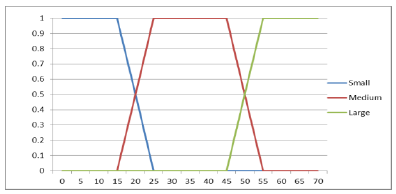
\includegraphics[width=8cm]{gambar2diagramfuzifikasidet.png}
    \caption{Diagram Fuzifikasi DET pada ILF dan EIF}
    \label{gb2}
\end{figure}

\begin{figure}[H]
    \centering
    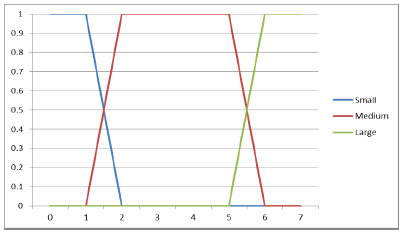
\includegraphics[width=8cm]{gambar3diagramfuzifikasiret.png}
    \caption{Diagram Fuzifikasi RET pada ILF dan EIF}
    \label{gb3}
\end{figure}

\begin{figure}[H]
    \centering
    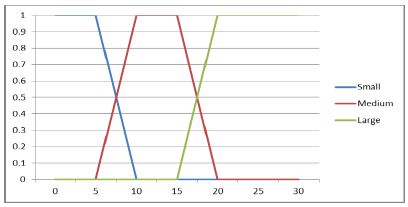
\includegraphics[width=8cm]{gambar4diagramfuzifikasidet.png}
    \caption{Diagram Fuzifikasi DET pada EI}
    \label{gb4}
\end{figure}

\begin{figure}[H]
    \centering
    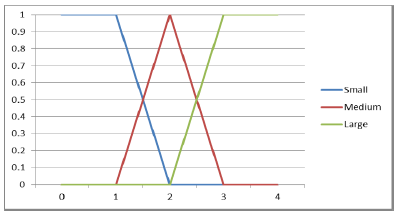
\includegraphics[width=8cm]{gambar5diagramfuzifikasiret.png}
    \caption{Diagram Fuzifikasi RET pada EI}
    \label{gb5}
\end{figure}

\begin{figure}[H]
    \centering
    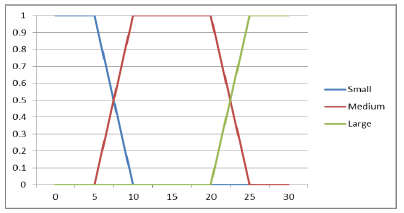
\includegraphics[width=8cm]{gambar6diagramfuzifikasidet.png}
    \caption{Diagram Fuzifikasi DET pada EO dan EQ}
    \label{gb6}
\end{figure}

\begin{figure}[H]
    \centering
    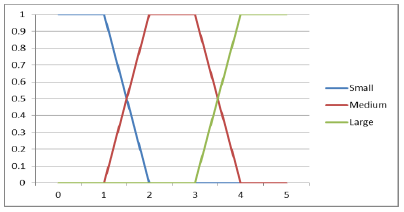
\includegraphics[width=8cm]{gambar7diagramfuzifikasiret.png}
    \caption{Diagram Fuzifikasi RET pada EO dan EQ}
    \label{gb7}
\end{figure}

\par Dengan menggunakan metode Mamdani sebagai \textit{Fuzzy Inference System} maka output dalam proses defuzzifikasi berupa nilai \textit{range}, seperti yang ditunjukan oleh beberapa gambar dibawah ini.

\begin{figure}[H]
    \centering
    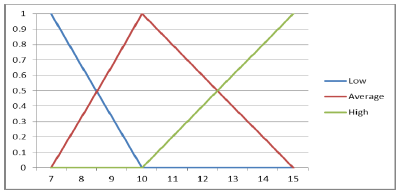
\includegraphics[width=8cm]{gambar8diagramdefuzifikasi.png}
    \caption{Diagram Defuzifikasi pada ILF}
    \label{gb8}
\end{figure}

\begin{figure}[H]
    \centering
    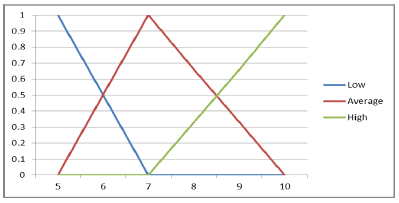
\includegraphics[width=8cm]{gambar9diagramdefuzifikasi.png}
    \caption{Diagram Defuzifikasi pada EIF}
    \label{gb9}
\end{figure}

\begin{figure}[H]
    \centering
    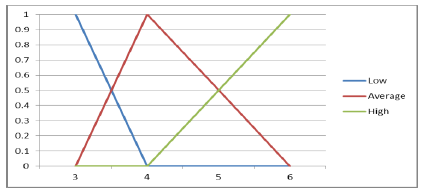
\includegraphics[width=8cm]{gambar10diagramdefuzifikasi.png}
    \caption{Diagram Defuzifikasi pada EI dan EQ}
    \label{gb10}
\end{figure}

\begin{figure}[H]
    \centering
    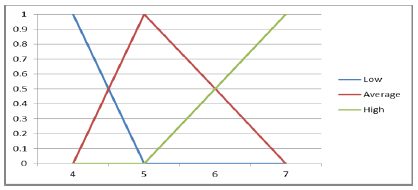
\includegraphics[width=8cm]{gambar11diagramdefuzifikasi.png}
    \caption{Diagram Defuzifikasi pada EO}
    \label{gb11}
\end{figure}

\par Untuk hasil LOC dari metode FPA dengan \textit{fuzzy logic} seperti terlihat pada tabel 8.

\begin{table}[H]
    \centering
    \caption{LOC dengan Metode FPA Menggunakan Fuzzy Logic}
    \bigskip
    \begin{tabular}{|c|c|}
        \hline
        \textbf{Aplikasi} & \textbf{LOC (\textit{lines})}\\
        \hline
        Akomodasi & 4008.23\\
        Avenger & 2441.97\\
        Catering & 3855.92\\
        IMB & 3374.34\\
        iSpeedy & 5217.81\\
        Meetingroom & 3507.79\\
        \hline
    \end{tabular}
    \label{tab8}
\end{table}

\subsection{Pembandingan Hasil}

\par Setelah semua hasil LOC didapat dari metode FPA dan \textit{fuzzy logic} maka dilakukan pembandingan hasil diantara semua metode tersebut, dengan cara mencari nilai \textit{Mean Absolute Error} (MAE) dari selisih nilai LOC yang didapat dari metode FPA dan \textit{fuzzy logic} dengan nilai LOC real yang didapat dari \textit{software SLOC Metrics} 3.0. Hasil MAE untuk setiap metode seperti terlihat di tabel 9.

\begin{table}[H]
    \centering
    \caption{LOC dengan Metode FPA Menggunakan Fuzzy Logic}
    \bigskip
    \begin{tabular}{|c|c|}
        \hline
        \textbf{Metode} & \textbf{MAE (\textit{lines})}\\
        \hline
        FPA & 154.82\\
        \textit{Fuzzy Logic} & 93.437\\
        \hline
    \end{tabular}
    \label{tab9}
\end{table}

% Penutup
\section{PENUTUP}

\subsection{Kesimpulan}

\par Metode \textit{Software Size Estimation} tidak ada yang memberikan tingkat akurasi sebesar 100 persen, dengan penambahan metode \textit{software engineering}.

\subsection{Saran}

\par Penggunaan metode \textit{software engineering} pada FPA untuk memprediksi size sebuah aplikasi tidak terbatas pada \textit{fuzzy logic.} Sebagai contoh, terdapat \textit{Artificial Intelligent System} yang menggunakan data penghitungan sebelumnya sebagai nilai pembanding untuk hasil yang dikeluarkan. 

\par Selain itu dengan dihasilkannya nilai FP maka mendapatkan estimasi perangkat lunak tidak hanya terbatas pada LOC. Dengan nilai FP bisa didapat pula biaya, waktu pengerjaan, dan sumber daya yang harus dikeluarkan agar proses pengerjaan sebuah proyek perangkat lunak akan berjalan efektif dan efisien. Perlu dilakukan penelitian untuk mendapatkan nilai estimasi selain LOC dengan menggunakan FP.

% Referensi
\bibliographystyle{apalike}
\bibliography{referensi}

\end{multicols}

\end{document}